\documentclass{ifaPoster}

\usepackage[utf8]{inputenc}
\usepackage[ngerman]{babel}
\usepackage{blindtext}
\usepackage{amsmath} % für multline
%\usepackage{subfig} % für subfloat
\usepackage{todonotes}

\ifaAuthor{Meret Feldkemper}
\ifaTitle{Kollaborative Problemlösung in modularen Anlagen mittels persönlicher digitaler Assistenz}
\ifaSupervisorA{Dipl.-Ing. Sebastian Heinze}
%\ifaSupervisorB{Dipl.-Ing. Betreuer B}
%\ifaSupervisorC{Dipl.-Ing. Betreuer C}
\ifaProfessor{Prof. Dr.-Ing. habl. Leon Urbas}
\ifaDayOfSubmission{02.05.2019}
\ifaThesis{Diplomarbeit}
\ifaPhoto{DA_files/Passbild.jpg}
 
\begin{document}

\section{Motivation}
Durch Voranschreiten der Automatisierung sind Anlagenbediener vor allem in kritischen Situationen für Entscheidungen verantwortlich \cite{bainbridget_ironies_1983}. Der Mensch trifft seine Entscheidungen anhand von Beobachtungen und Erfahrungen. Im Zuge der entwickelten Modularisierungskonzepte für die Prozessindustrie wird dies zunehmend schwieriger. Die Flexibilität der modularen Anlagen stellt die Anlagenbediener vor die Herausforderung, Probleme nicht mehr auf Grundlage von umfangreicher Erfahrung lösen zu können \cite{mueller_2018}. Assistenzsysteme können den Anlagenbediener bei Erkennung von Problemen, deren Zusammenhängen und möglichen Lösungsansätzen Unterstützung bieten. 
%Dabei ist der Mensch mit einzubeziehen und seine Kompetenzen zu würdigen.

Für ein Assistenzsystem in modularen Anlagen wurde zunächst identifiziert, welche Faktoren bei der Entwicklung zu berücksichtigen sind. Darauf basiert das Konzept für die Nutzeroberfläche, die zwischen Assistenz und Nutzer kommuniziert (siehe Abbildung \ref{Assistenzsystem}).

\begin{figure}[htbp]
\centering
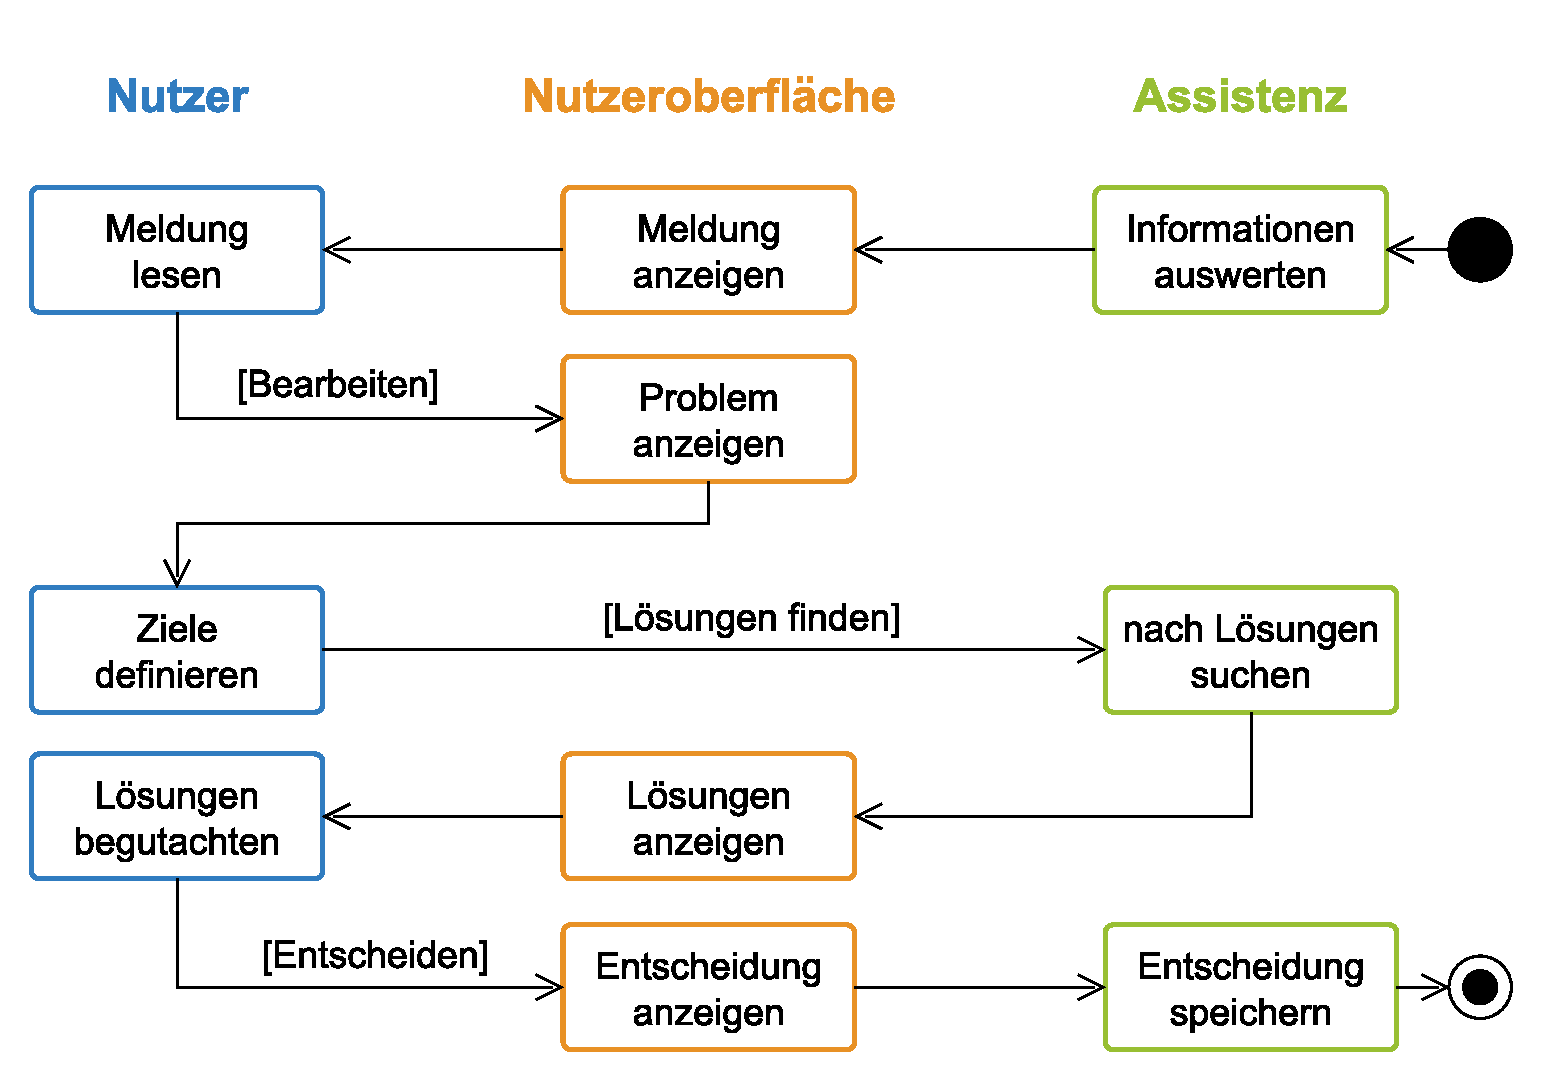
\includegraphics[scale=0.67]{DA_files/Ablauf-Assistenzsystem.pdf}
\caption{Nutzer und Assistenz kollaborieren mithilfe der Nutzeroberfläche}
\label{Assistenzsystem}
\end{figure}

\section{Analyse}
Tritt in der modularen Anlage ein Problem auf, muss der Nutzer darauf aufmerksam gemacht werden. Wichtig für die Assistenz ist nicht nur die Problemursache einzuordnen, sondern auch wie zeitkritisch und komplex das Problem ist. Anhand dieser Merkmale soll sich die Menge und Art der dargestellten Informationen orientieren.
%Aktuell erhält der Nutzer mit der Prozessführungsebene (PFE) nur eine Gesamtübersicht über den aktuellen Zustand der Anlage. Treten Meldungen auf, wird dem Nutzer nicht sichtbar gemacht, welcher Bereich betroffen ist und wie die Zusammenhänge sind.

Sollen Lösungen für ein entstandenes Problem gefunden werden, sind vor allem die Ziele eines produzierenden Unternehmens zu berücksichtigen.
Diese reichen von der Verfügbarkeit von Mitarbeitern bis zum Aufwand Änderungen an der Anlage vorzunehmen.
%Diese reichen von der Verfügbarkeit von Mitarbeitern bis zum Aufwand Änderungen an der Anlage vorzunehmen.

\section{Konzept}
Die entwickelte Nutzeroberfläche baut auf einer bereits entwickelten Prozessführungsebene (PFE) auf und begleitet den Nutzer durch den Problemlöseprozess. Die Anpassung an den Problembereich wurde integriert, indem irrelevante Informationen versteckt werden. Der Nutzer kann, durch die Anpassung der Ziele an die aktuellen Bedingungen im Unternehmen, den Problemlöseprozess steuern. Anhand der eingegebenen Spezifikationen sucht das Assistenzsystem dann nach Lösungsmöglichkeiten, die dem Nutzer sowohl visuell als auch zahlenmäßig dargestellt werden (siehe Abbildung \ref{PFE-Loesungen}). Diese Angaben sollen eine Entscheidung erleichtern.
\begin{figure}[htbp]
\centering
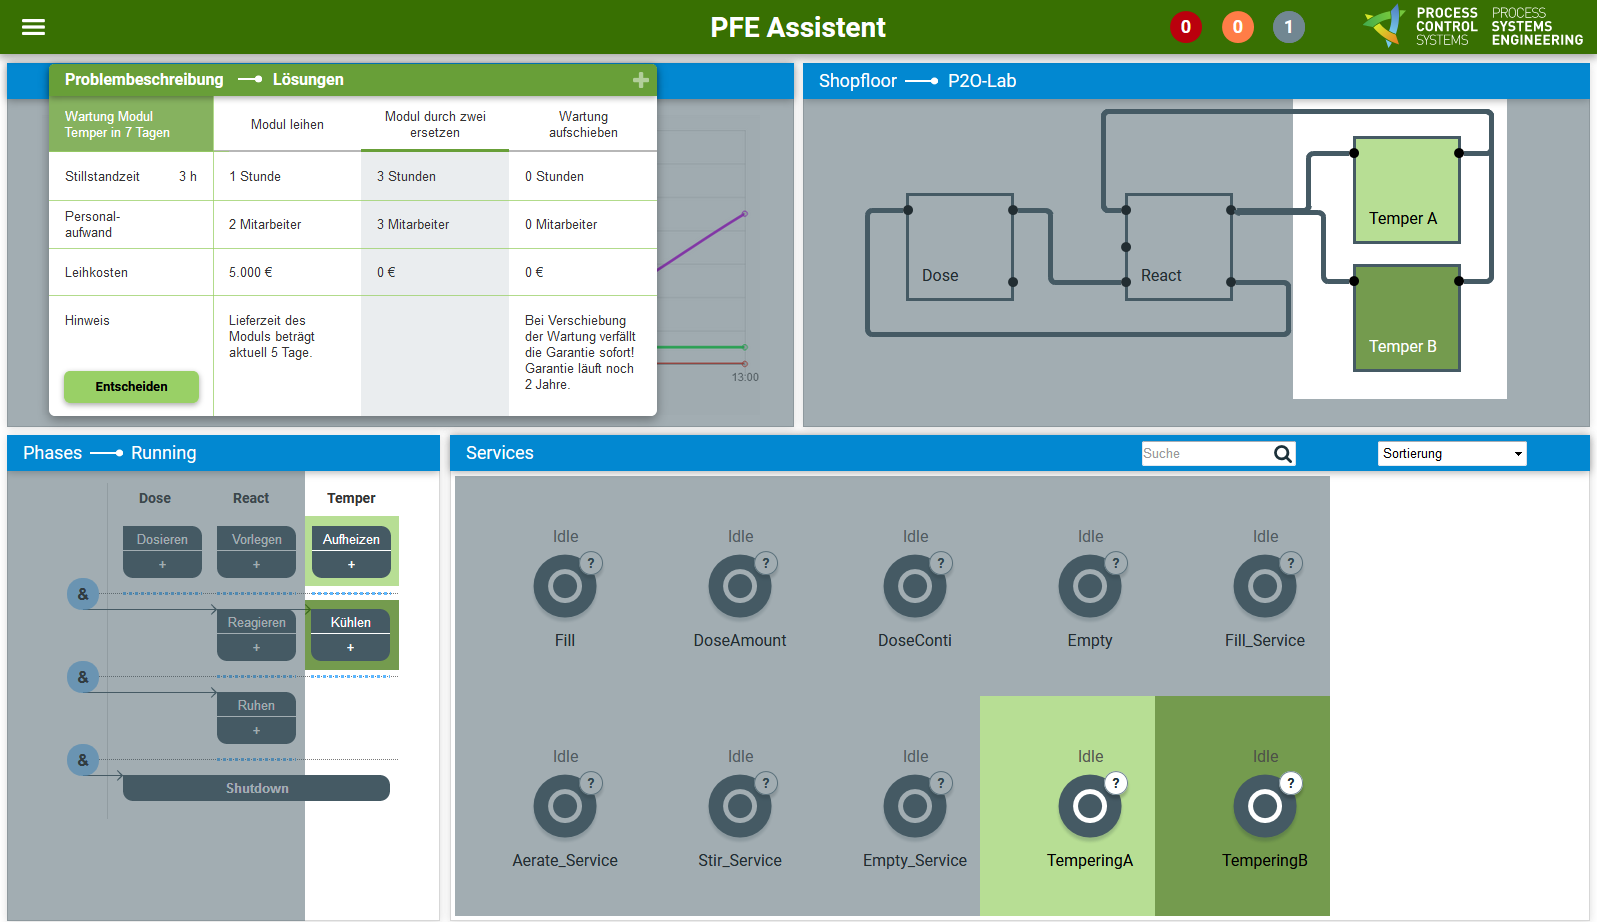
\includegraphics[scale=0.42]{DA_files/Prototyp-PFE-Loesung2.png}
\caption{Darstellung einer Lösung für ein Problem auf Grundlage der PFE}
\label{PFE-Loesungen}
\end{figure}

\section{Validierung}
Zur Beurteilung der entwickelten Nutzeroberfläche erfolgte eine Umfrage unter Experten, welche mit den Bedienkonzepten modularer Analgen vertraut sind. Positiv hervorgehoben wurde der schlichte Aufbau, die Übersichtlichkeit und die einfache Bedienung. Der Automatisierungsgrad des Assistenten überzeugt mit einer angemessenen Auswahl an Zielen und Lösungen. Verbesserungspotential besteht bei der detaillierten Darstellung der Lösungen. Es wird einheitlich eine Angabe der Gesamtkosten, die bei Anwendung der Lösung entstehen, gewünscht. Aufgrund des insgesamt überzeugenden Konzepts wird eine Implementierung der Nutzeroberfläche von den Experten unterstützt.

%Die Umfrage unter Experten ergab, dass die Entscheidung zwar erleichtert wird, sie jedoch immer noch schwierig ist. Sie wünschen sich einheitlich die Angabe von Gesamtkosten, die bei Anwendung der Lösung entstehen. Dadurch erhoffen sie sich eine bessere Vergleichbarkeit der einzelnen Lösungen. Insgesamt wurde der Automatisierungsgrad des Assistenten positiv bewertet. Die Auswahl an Zielen und Lösungen ist, laut der Experten, angemessen, da diese den Nutzer gut leiten. Aufgrund des schlichten Aufbaus, der Übersichtlichkeit und der einfachen Bedienung wird die Nutzeroberfläche von den Experten empfohlen. 
%Für eine konkrete Anwendung der Nutzeroberfläche wird zudem gewünscht, den Nutzer auch bei der Durchführung der Lösung zu unterstützen.
%Die Befragung einiger Experten zu dem vorgestellten Prototypen ergab ein insgesamt positive Bewertung. Sie schätzen insbesondere die gute Übersichtlichkeit und einfache Bedienung des Assistenzsystems. Besonders hervorgehoben wurde die Tatsache, dass die Assistenz bereits eine Vorauswahl an möglichen Zielen und Lösungen trifft. Dadurch wird der Nutzer nicht mit zu vielen Informationen überfordert. 


\section{Zusammenfassung und Ausblick}
Der Anlagenbediener wird mit dem Assistenzsystem durch die Phasen des Problemlöseprozesses begleitet. Die Nutzeroberfläche stellt die Probleme und Lösungen dar und dient zur Kommunikation zwischen Mensch und Assistenz. Die Assistenz analysiert im Hintergrund die vorhandenen Informationen und teilt sie dem Nutzer über die Nutzeroberfläche mit. Dadurch entsteht ein kollaborativer Problemlöseprozess. Die Auswertung der Umfrage zeigt, dass die Nutzeroberfläche, bei Erweiterung um ein intelligentes System, Anwendung findet.

%Offen bleibt, wie der Nutzer selber Probleme und Lösungen eingeben kann.
Mit der entwickelten Nutzeroberfläche kann nun untersucht werden, welchen Einfluss die Menge der Informationen über Problem und Lösung auf die Entscheidung des Anlagenbediener hat. Darauf aufbauend sollten Schnittstellen im Modul Type Package geschaffen werden, damit die Anwendung des Assistenzsystems möglich ist.

\vspace{8pt}
 {\tiny\renewcommand{\section}[2]{}%
 	 \begin{thebibliography}{8.5}
 	 \bibitem{bainbridget_ironies_1983}
 	 	Lisanne Bainbridget. {\glqq Ironies of Automation\grqq}. {In: \textit{Automatica}} 19.6 (1983), S. 775-779.
 	 \bibitem{mueller_2018}
 	 Romy Müller. {\glqq Cognitive challenges of changeability: adjustment
to system changes and transfer of knowledge in modular
chemical plants\grqq}. {In: \textit{Cognition, Technology and Work}} 21.1 (2018), S. 113-131.
	\end{thebibliography}}
	
\end{document}